% This must be in the first 5 lines to tell arXiv to use pdfLaTeX, which is strongly recommended.
\pdfoutput=1
% In particular, the hyperref package requires pdfLaTeX in order to break URLs across lines.

\documentclass[12pt]{article}

% Remove the "review" option to generate the final version.
\usepackage[review]{ACL2023}

% Standard package includes
\usepackage{times}
\usepackage{latexsym}

% For proper rendering and hyphenation of words containing Latin characters (including in bib files)
\usepackage[T1]{fontenc}
% For Vietnamese characters
% \usepackage[T5]{fontenc}
% See https://www.latex-project.org/help/documentation/encguide.pdf for other character sets

% This assumes your files are encoded as UTF8
\usepackage[utf8]{inputenc}

% This is not strictly necessary, and may be commented out.
% However, it will improve the layout of the manuscript,
% and will typically save some space.
\usepackage{microtype}

% This is also not strictly necessary, and may be commented out.
% However, it will improve the aesthetics of text in
% the typewriter font.
\usepackage{inconsolata}
\usepackage{graphicx}
\usepackage{float}
\usepackage{booktabs} % For better table formatting
\usepackage{multirow}
\usepackage{array}

% If the title and author information does not fit in the area allocated, uncomment the following
%
%\setlength\titlebox{<dim>}
%
% and set <dim> to something 5cm or larger.

\title{Harnessing Ensemble Learning to Shape Consumer Choices: A Yelp Sentiment Analysis Approach}

\author{Nomita Chandra \and Kevin Kuc \and Weijie Yang \\
        nchandra4@berkeley.edu \\ kkuc100@berkeley.edu \\ raphaelyang1998@berkeley.edu}

\begin{document}
\maketitle
\begin{abstract}
  In the current digital landscape, online presence and customer reviews play a crucial role in shaping consumer perceptions and influencing purchasing decisions. Platforms such as Yelp have become essential, offering a comprehensive medium for consumers to discover, connect with, and transact with local businesses. This increased reliance on Yelp reviews has significantly impacted business reputations and success. Consequently, the growing volume of reviews necessitates the development of efficient and accurate methods for their analysis. In this paper, we proposed to perform sentiment classification on Yelp reviews using the \href{https://huggingface.co/datasets/Yelp/yelp_review_full}{Yelp Review Dataset} from Hugging Face, originally constructed by Xiang Zhang from the Yelp Dataset Challenge 2015. We utilized the Yelp Review Dataset, comprising 650,000 training and 50,000 test reviews labeled from 1 to 5 stars. Sentiment analysis of customer reviews was crucial for businesses to gauge customer satisfaction, identify improvement areas, enhance customer experiences, address negative feedback promptly, and reinforce positive service aspects. We employed RoBERTa, Bert-large-uncased, and Flan-T5 as base models, leveraging Ensemble Learning to enhance model performance. RoBERTa’s Masked Language Modeling (MLM) enabled comprehensive information extraction, Bert-large-uncased’s bi-directional training approach considered both left and right contextual information, and Flan-T5’s encoder extracted semantic meanings to facilitate inference. Ensemble Learning integrated the outputs of these models, as illustrated in the algorithmic architecture. [Details on the methods used for testing will be outlined here.] [Results of the sentiment classification testing will be presented here.]
\end{abstract}


\section{Introduction}
In today’s digital era, a business's online presence and customer reviews play a crucial role in shaping consumer perceptions and driving purchasing decisions\footnote{Luca, M. (2016). Reviews, Reputation, and Revenue: The Case of Yelp.com. Harvard Business School Working Paper.}. Yelp, a prominent platform for discovering, connecting with, and transacting with local businesses, serves as a key resource for consumers seeking accurate information to guide their choices \citep{lee2014impact}. With its significant impact on consumer behavior, businesses worldwide strive to achieve higher ratings and positive feedback. As the volume of reviews continues to grow, the demand for efficient and precise methods to analyze and classify this textual data has never been greater \citep{pang2008sentiment}.

\subsection{Importance}
Our project, "Harnessing Ensemble Learning to Shape Consumer Choices: A Yelp Sentiment Analysis Approach" focuses on classifying the sentiment of Yelp reviews. Utilizing the Yelp Review Dataset from Hugging Face, originally curated by Xiang Zhang during the Yelp Dataset Challenge 2015 \citep{zhang2015sensitivity}, our model is designed to infer sentiment ratings for Yelp reviews. Understanding customer sentiment is vital for businesses, as it provides insights into customer satisfaction, highlights areas for improvement, and helps address feedback effectively \citep{jurafsky2020speech}. By leveraging sentiment analysis, businesses can enhance customer experiences, promptly address negative comments, and reinforce positive aspects of their services \citep{pang2008sentiment}.

\section{Background}
Sentiment analysis is defined as associating text to positive, neutral or negative sentiment and is crucial in today's world for understanding emotional motivations. This type of insight is revolutionizing market research as we can use it to predict future consumer actions\footnote{ConvergeHub, \textit{Six Principles for Knowing Your Customers Better}.}. However, sentiment analysis is more challenging than expected due to the subjective nature of opinions and interpretations of sentiment. Since this type of classification relies heavily on individual perspectives, the "correct" label can vary depending on who is classifying the text. As a result, there may not be a consensus on the sentiment label.

In this research paper, we will be focusing on the machine learning-based approach for text sentiment extraction, which uses labeled text instances to build classifiers. Common approaches to semantic analysis involve supervised methods, which require texts labeled with sentiment categories like positive, negative, or neutral. In supervised learning, the model learns to map input features to labeled outputs by adjusting parameters to define decision boundaries that separate classes, enabling it to make accurate predictions on new, unseen data. Examples of supervised models include decision trees, Naive Bayes, neural networks, support vector machines (SVMs), and k-nearest neighbors (KNNs) \citep{dankhara2022}. Naive Bayes uses a bag-of-words model where text is represented by predefined word counts or frequencies, treating each feature independently and estimating class probabilities using Bayes' theorem while assuming feature independence.

The sentiment classifiers provided by Pang et al. \citep{pang2008sentiment} on a movie review dataset demonstrated the validity and capability of Naive Bayes, maximum entropy, and SVM in text categorization. Although, we see that the dominant model techniques within sentiment analysis follow a topical approach not taking into account semantic relationships between words. In this research paper, we want to use these dominant techniques like Naive Bayes and use them as a baseline as we explore different architectures like Transformer-based Models \citep{kokab2022transformer}. These models leverage self-attention mechanisms to weigh the importance of different words in a sentence, allowing them to understand context and nuance more effectively than traditional methods. They are pre-trained on large corpora of text and can be fine-tuned for specific tasks, which makes them highly adaptable. Transformer models learn dynamic, context-aware features during pre-training, which can adapt to various tasks and domains. In contrast, Naive Bayes uses fixed probabilistic features and SVMs rely on static feature representations. 


\subsection{Challenges}
One of the primary challenges in our project is preprocessing the data to ensure its relevance and usability for sentiment analysis. The dataset consists of reviews of varying lengths, necessitating the truncation and padding of reviews to create uniform input sizes while preserving their sentiment. Additionally, we need to consider implementing data augmentation techniques to expand our dataset, enabling our model to train on a larger and more diverse set of data. Lastly, a significant challenge is developing the machine learning model's capability to extract semantic meaning from lengthy reviews.

\subsection{Dataset}
We utilized the \href{https://huggingface.co/datasets/Yelp/yelp_review_full}{Yelp Review Dataset} available on Hugging Face, which is constructed by randomly taking 130,000 training samples and 10,000 testing samples for each review star from 1 to 5. In total there are 650,000 trainig samples and 50,000 testing samples. For our analysis, we considered three distinct data configurations:

\begin{itemize}
  \item \textbf{Original Five-Class Classification:} We analyzed the dataset with its original five-star rating scale. This approach is anticipated to have the lowest accuracy due to the inherent difficulty in distinguishing between closely related classes, such as between 1 and 2 stars, as well as between 4 and 5 stars.

  \item \textbf{Three-Class Classification:} We reclassified the reviews into three categories: 'negative' for 1-2 stars, 'positive' for 4-5 stars, and 'mixed' for 3 stars. Reviews with 1-2 stars were grouped together as they predominantly contain negative critiques, while 4-5 stars generally reflect positive feedback. Reviews with a 3-star rating represent a mix of both positive and negative observations. This approach is expected to yield intermediate accuracy, as it simplifies the classification task compared to the original five-class problem.

  \item \textbf{Binary Classification:} We reclassified the reviews into two categories: 'negative' for 1-2 stars and 'positive' for 4-5 stars, excluding 3-star reviews from the dataset. This binary classification is hypothesized to provide the highest accuracy, as it removes the ambiguity associated with the 'mixed' category.
\end{itemize}

\section{Methodology}
This section describes our approach, including data processing, complete model architecture as well as output summarization technique for applications.

% Methodology image inclusion
\begin{figure}[H]
  \centering
  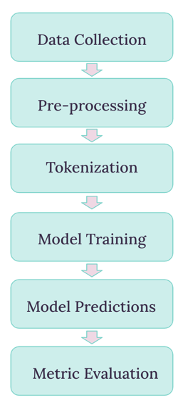
\includegraphics[width=0.2\textwidth, height=0.3\textheight]{./methodology.jpg}
  \caption{Comprehensive overview of our approach, detailing each stage from Data Collection through Metric Evaluation.}
  \label{fig:methedology}
\end{figure}

\section{Methods}

\subsection{Data Processing}
To prepare the Yelp Review Dataset for analysis, several preprocessing steps were conducted to ensure data quality and balance. Initially, the dataset, sourced from Hugging Face, was subjected to word count computation for each review. Reviews with word counts fewer than 100 or more than 200 were excluded. This range was chosen to filter out reviews that were too short, which often signify low-quality content, and overly lengthy reviews, which can introduce noise and complexity without providing additional value \citep{pang2008sentiment}. Following this, to create a balanced training and test set, random sampling was applied to select an equal number of samples from each label. These preprocessing steps were critical and necessary in ensuring that the dataset was of high quality, balanced, and representative of various sentiment categories, thus facilitating more accurate and reliable analysis and model training.

\subsection{Tokenization}
In sentiment analysis, tokenization transforms raw text into a structured format for processing, ensuring accurate representation of context and word variations. The tokenizers used—BertTokenizer, DebertaTokenizer, and RobertaTokenizer from the Hugging Face Transformers library—are each tailored to their respective model architectures. BertTokenizer is for the BERT model and employs WordPiece tokenization which splits words into characters and subwords. It uses special tokens like [CLS], [SEP], [PAD], and [MASK] to denote the start, separation, padding, and masking. The DebertaTokenizer, associated with the DebertaTokenizer, is designed for the DeBERTa model and uses SentencePiece tokenization. This approach processes input into subwords, efficiently handling out-of-vocabulary words while also using special tokens similar to those in BERT. RobertaTokenizer, used with the RoBERTa model, utilize special tokens like [CLS], [SEP], [PAD], and [MASK] to denote the start, separation, padding, and masking pairs of sequences to create subwords, and employs special tokens such as <s> for the start of a sequence, </s> for separation, <pad> for padding, and <mask> for masking. 

\subsection{Baseline Model}
To establish a foundational approach for classifying Yelp reviews, we implemented a bag-of-words (BoW) model in conjunction with a Naive Bayes classifier. This approach was chosen for its balance of simplicity and effectiveness in initial evaluations \citep{rish2001empirical}. The Naive Bayes classifier, grounded in Bayes' Theorem, is renowned for its computational efficiency and rapid processing capabilities. The model operates by tokenizing the text into individual words, which are then represented as discrete features. Each word token contributes to the calculation of the posterior probability of a given sentiment class based on its frequency and the class's prior probability. The Naive Bayes algorithm combines these token-based probabilities to infer the sentiment of the entire review. Given that reviewers often infuse their text with a high degree of passion and emotion, we anticipated that this approach would yield accurate results, as the BoW model is well-suited to capture these sentiments through the frequency and presence of emotionally charged words.

\subsection{Upstream Base Model Selection}
For the classification tasks, we employed RoBERTa (Robustly optimized BERT approach) and DeBERTa (Decoding-enhanced BERT with disentangled attention) as our upstream base models for the whole model architecture. We take the hidden layers from both two BERT models and connected with dense layers as well as a softmax layer for our downstream classification task. 

\subsection{RoBERTa}
RoBERTa is an enhanced version of BERT that has been optimized through longer training with larger batches, removal of the next sentence prediction objective, and training on a larger dataset \citep{liu2012sentiment}. These improvements enable RoBERTa to achieve superior performance by better capturing the nuances of language, making it particularly suitable for sentiment analysis and text classification tasks where understanding context and sentiment from text is crucial \citep{liu2012sentiment}. We expect that Its great capabilities in sentiment comprehension can identify people’s preferences and attitudes entailed in the reviews and generate predictions with qualities.

\subsection{DeBERTa}
DeBERTa introduces disentangled attention mechanisms and an enhanced mask decoder, which allow it to more effectively encode semantic information and improve the model's performance on downstream tasks \citep{he2020deberta}. The disentangled attention mechanism separates the content and position information, leading to a more refined understanding of the text, which is beneficial for accurately classifying reviews that may have subtle sentiment cues \citep{he2020deberta}. Subtle sentiment detection ability is crucial to our task as we classify the review in a star-rating model. It is easy to identiy “star 0” and “star 4”. However, the boundary and difference between “star 0” and “star 1” is ambiguous as they both show negative sentiment signals in reviews. How to define the degree of negative sentiment requires high sensitivity to subtle sentiment change for the model.

By leveraging the strengths of RoBERTa and DeBERTa, we aimed to enhance the predictive performance and reliability of our classification models, ensuring they could handle the complexities of the Yelp Review Dataset effectively. Besides, we employed the Text-to-Text Transfer Transformer (T5) model for summarizing our modeling results. The T5 model transforms all NLP tasks into a text-to-text format, including summarization. Its strength lies in its extensive pre-training, allowing it to generate coherent and concise summaries. From the perspective of users who care about the reviews and hope to gain insights from the reviews to improve the products as well as mitigate existing issues, our who model architecture and solution needs to generate summarized outputs to highlight the key useful information to the users instead of passing them long reviews.

\subsection{Ensemble}
Ensemble learning is an effective approach to mitigate overfitting by averaging biases and variances from multiple models, thus enhancing overall model performance \citep{opitz1999popular}. It also corrects the errors made by individual weak learners, leading to better predictive accuracy \citep{schapire1990strength}. Figure 2 displays our whole model architecture. First, we preprocessed the dataset and tokenized the dataset with DeBERTa and RoBERTa’s tokenizers correspondingly. Then, we customized both BERT models by taking their hidden states and importing to dense layers and softmax layers to get the predictions. To better integrate and boost the prediction capbilities, as well as taking the strength of both BERT models, we employed multiple Ensemble Learning approaches including averaging, stacking, voting, MLP, random forest, decision tree, and gradient boosting. Specifically, we take the softmax layers with the size of [5*batch size] from both two models and compute the average value of the two vectors as the input for ensemble learning classifier to get the final prediction. Above models are fine-tuned to get the best performance version. Then, T5 is adopted here to take the outputs for each class and summarize the long reviews into short sentences and keywords.

% Model_architecture image inclusion
\begin{figure*}[h!]
  \centering
  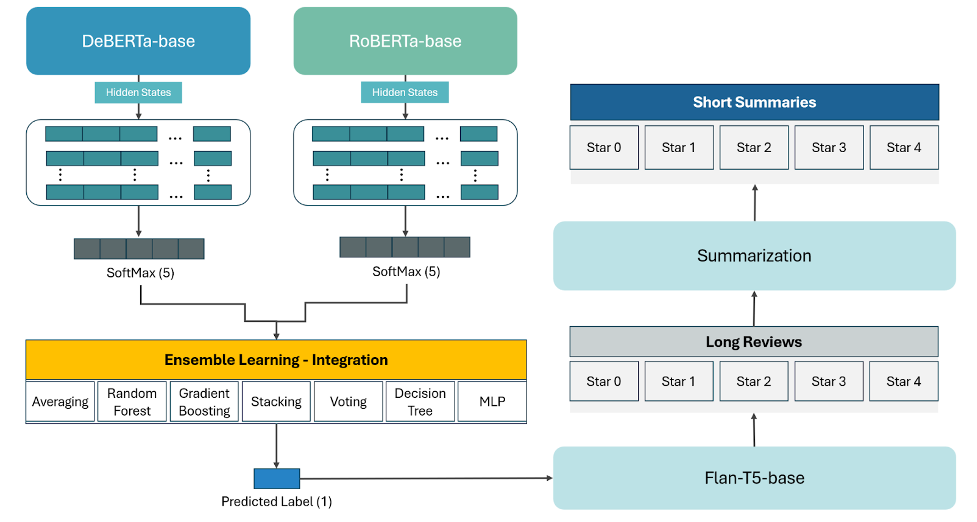
\includegraphics[width=1.0\textwidth, height=0.3\textheight]{./model_architecture.png}
  \caption{Whole model architecture by using ensemble learning to consolidate the model predictions from both DeBERTa and RoBERTa base models.}
  \label{fig:model_architecture}
\end{figure*}

\begin{table*}[h!]
  \centering
  \small % Reduces the font size
  \begin{tabular}{|p{3cm}|p{4.7cm}|>{\centering\arraybackslash}p{1.5cm}|>{\centering\arraybackslash}p{1.5cm}|>{\centering\arraybackslash}p{1.5cm}|>{\centering\arraybackslash}p{1.5cm}|}
    \hline
    \textbf{Model} & \textbf{Best Training Hyperparameters} & \textbf{Test set Macro F1} & \textbf{Test set Micro F1} & \textbf{Test set Precision} & \textbf{Test set Recall} \\
    \hline
    Naive Bayes (Baseline) & - & 0.53 & 0.53 & 0.53 & 0.53 \\
    \hline
    RoBERTa-base (Customized) & \begin{tabular}[c]{@{}l@{}}Learning rate: 1e-5 \\ Hidden layers size: 100 \\ Dropout: 0.20 \\ Max length: 200 \\ Epochs: 4\end{tabular} & 0.58 & 0.58 & 0.59 & 0.58 \\
    \hline
    DeBERTa-base (Customized) & \begin{tabular}[c]{@{}l@{}}Learning rate: 1e-5 \\ Hidden layers: 200 \\ Dropout: 0.20 \\ Max length: 200 \\ Epochs: 3\end{tabular} & 0.58 & 0.58 & 0.62 & 0.58 \\
    \hline
    Ensemble Learning (Averaging) & - & 0.59 & 0.59 & 0.61 & 0.59 \\
    \hline
    \textbf{Ensemble Learning (Random Forest)} & \textbf{Max depth: 2} & \textbf{0.62} & \textbf{0.62} & \textbf{0.63} & \textbf{0.62} \\
    \hline
    Ensemble Learning (Decision Tree) & Max depth: 3 & 0.61 & 0.61 & 0.62 & 0.61 \\
    \hline
    \textbf{Ensemble Learning (MLP)} & \textbf{\begin{tabular}[c]{@{}l@{}}Max iterations: 500 \\ Learning rate: 0.005\end{tabular}} & \textbf{0.62} & \textbf{0.62} & \textbf{0.62} & \textbf{0.62} \\
    \hline
    Ensemble Learning (Gradient Boosting) & \begin{tabular}[c]{@{}l@{}}Estimators: 200 \\ Learning rate: 0.005\end{tabular} & 0.58 & 0.58 & 0.59 & 0.58 \\
    \hline
    Ensemble Learning (Stacking) & \begin{tabular}[c]{@{}l@{}}Random Forest (estimators: 10) \\ MLP (max iterations: 500, \\ learning rate: 0.005) \\ Gradient Boosting (estimators: 200, \\ learning rate: 0.005)\end{tabular} & 0.55 & 0.55 & 0.57 & 0.55 \\
    \hline
    Ensemble Learning (Voting) & \begin{tabular}[c]{@{}l@{}}Random Forest (estimators: 10) \\ MLP (max iterations: 500, \\ learning rate: 0.005) \\ Gradient Boosting (estimators: 200, \\ learning rate: 0.005)\end{tabular} & 0.61 & 0.60 & 0.61 & 0.60 \\
    \hline
  \end{tabular}
  \caption{5 class grid search result for baseline model, BERT models, and ensemble learning.}
  \label{tab:model_performance}
\end{table*}


\section{Results and Discussion}
We conducted a grid search, experimenting with different hyperparameter sets to identify the best performing models for Naive Bayes (baseline), RoBERTa-base, and DeBERTa-base. After determining the optimal BERT models, we explored various ensemble learning approaches, including averaging, stacking, voting, random forest, decision tree, and multi-layer perceptrons, to identify the top ensemble performers. This section discusses three main aspects: upstream model performance, ensemble learning, and T5 summarization.

Table 1 displays our grid search results. To ensure the robustness of our experiments, we first conducted modeling with three classes to evaluate model performance and then extended it to five classes. Overall, our model pipeline achieved 79 percent in both Macro F1 and Micro F1 scores for the three-class classification, which is significantly higher than the baseline model for 0.68 percent. For the five-class task, our fine-tuned model achieved 62 percent in both Macro F1 and Micro F1 scores using MLP and Random Forest approaches by consolidating the softmax outputs from RoBERTa-base and DeBERTa-base, also significantly higher than the baseline model by 0.53 percent. Next, we provide a detailed analysis of the performance at the class level for each model and approach.

\subsection{Baseline Results}
Our results demonstrated the model’s performance across different classification schemes. For the original five-class classification, the BoW model achieved an accuracy of 0.52, with stars 1 and 2 exhibiting the lowest F1-scores of 0.44 and 0.47, respectively. In the three-class classification, the model achieved an accuracy of 0.68, though the neutral class had the lowest F1-score of 0.61. The binary classification model performed notably better, with an accuracy of 0.88, and both categories showed equal accuracy. The assumption of feature independence allows for straightforward computation, but to further refine our model's performance, the next phase involved incorporating additional contextual information and exploring more sophisticated methods \citep{rish2001empirical}.

\subsection{RoBERTa-base and DeBERTa-base}
With multiple experiments to fine-tune the best model, Table 2 displays the details of two upstream models in five-class predictions. Overall, both models excel at predicting “Star 0” (most negative reviews). However, they exhibit different capabilities in the remaining classes.

\subsubsection{RoBERTa-base}
RoBERTa-base demonstrates its ability to identify the most negative and positive reviews, achieving 68 percent and 71 percent F1-scores for “Star 0” and “Star 4,” respectively, while DeBERTa-base only achieves a 52 percent F1-score for “Star 4.” The confusion matrix provides a detailed breakdown, revealing that RoBERTa has a strong classification capability for positive reviews, with a 62 percent recall rate for “Star 3.” However, the recall rate decreases when the reviews are negative, indicating that the model struggles more with these classes. Specifically, the “Star 1” class is particularly challenging for RoBERTa to define, with a recall rate of 36 percent. To illustrate this, we analyzed an example of a misclassification by RoBERTa-base.

\begin{itemize}
  \item \textbf{Miss Classification: ``Star 1'' Classified as ``Star 0''}
\end{itemize}

\begin{quote}“Great location, ok rooms, ok restaurants. Horrible staff. I felt like i was inconveniencing them by asking for simple directions. Incredibly rude and everyone looked like they were miserable. Probably the worst part of my experience was the Spa. Please avoid this hell hole even if they offer it to you for free! It is incredibly dirty and smells. I couldnt take more then 20 min and i left to take a long shower in my room. Try calling the front desk and youll wait anywhere from 10 to 20 minutes every time. There are SO many better hotels on the strip around the same price. I will not be staying here again!”
\end{quote}

This review is labeled as “Star 1,” but RoBERTa predicts it as “Star 0.” The model easily recognizes it as a negative review based on the overall content. However, the review actually mentions some positive aspects, such as the location, room, and restaurant. This is where DeBERTa's advantage becomes evident. With its ability to perceive subtle sentiment expressions, DeBERTa can recognize that the entire review is not wholly negative. It identifies some positive points mentioned early in the text. In contrast, RoBERTa tends to focus more on the overall sentiment, leading to an incorrect prediction.

\subsubsection{DeBERTa-base}
According to the above analysis, RoBERTa is sensitive to the most negative and positive reviews, while DeBERTa-base exhibits a relatively balanced performance among the classes, especially for “Star 1” to “Star 4,” with its consistent F1-scores (52 percent, 52 percent, 56 percent, 52 percent). This aligns with our expectation that DeBERTa can detect subtle sentiment differences among these classes, thereby achieving relatively good performance in overall classification accuracy. However, by examining its confusion matrix, we can see that its weakness lies in recognizing the most positive class, with only a 40 percent recall rate, compared to RoBERTa-base's 68 percent recall rate.

\begin{itemize}
  \item \textbf{Miss classification: “Star 4” classified as “Star 3”}
\end{itemize}

\begin{quote}“Their chips and salsa were quite good. The chips were served warm and they provided 3 types of salsas. I had the tostadas and they provided 3 full sized tostadas which were simply the best I've ever had in a restaurant.  My wife had a Vege Chimi which she loved.  It was light and crispy with a good mix of veges in it.  My daughter had the fish taco and beans which she enjoyed, although she didn't care for the dressing (1000 Island?) that came in it.  We finished the meal with some Sopapillas, which were wonderful as well. The service was warm, friendly and timely.  It's a pretty casual/comfortable place to go and we'll absolutely be back at Papi Chulo's the next time we're in Scottsdale. Not sure what's up with some of the negative reviews, but our experience was excellent all around and the food was very reasonably priced as well.”
\end{quote}

By examining the incorrect classifications of DeBERTa-base, an interesting finding emerges: the model seems overly sensitive to subtle sentiment expressions. DeBERTa assigns “Star 5” to reviews with strong positive tones and words such as “Love it!”, “Really great!”, or “Fantastic!” The example above is representative, where RoBERTa makes the correct prediction while DeBERTa does not. The review overall describes the customer’s experience in a relatively calm and rational tone but with full satisfaction. Although the content expresses positiveness, it lacks strong positive tones, such as exclamations. Consequently, DeBERTa tends to be conservative with such reviews, often judging them as “Star 4” instead of “Star 5.” This subtle sentiment sensitivity negatively impacts the model’s capability in classifying this category accurately.

Conclusively, although RoBERTa-base and DeBERTa-base have similar overall F1-score performance, their inference capabilities exhibit significant distinctions in specific class detections. RoBERTa-base is sensitive to the most negative and positive reviews, while DeBERTa-base excels at capturing subtle sentiment differences between classes, maintaining balanced scores in middle-class predictions. Therefore, we aim to integrate the strengths of both models to achieve a synergistic effect. To this end, ensemble learning was employed during the experimental stages, involving multiple classifier trials to determine the best method for consolidating the two models.

\subsection{Ensemble Learning}
To enhance our model's performance, we employed ensemble learning techniques using the RoBERTa and DeBERTa base models. We evaluated several methods to combine these models, including Averaging, Random Forest, Decision Tree, MLP (Multi-Layer Perceptron), Gradient Boosting, Stacking, and Voting. The results revealed that Random Forest and MLP achieved the highest performance scores, with Random Forest yielding an F1-score of 0.62 and MLP achieving an F1-score of 0.62. In contrast, Stacking produced the lowest performance score, with an F1-score of 0.55.

Random Forest achieved high performance with an F1-score of 0.62 due to its robust mechanism of aggregating predictions from multiple decision trees. Each decision tree in the Random Forest is trained on a bootstrap sample of the data, which introduces variability and helps capture different aspects of the dataset. For example, one decision tree might focus on features indicating strong sentiment, while another may identify subtle nuances in the text. By averaging the predictions of these trees, Random Forest effectively reduces the risk of overfitting and improves generalization, making it well-suited for the nuanced task of sentiment analysis in Yelp reviews.

MLP (Multi-Layer Perceptron), with an F1-score of 0.62, also performed well due to its ability to model complex relationships in the data. MLP employs multiple layers of neurons, where each layer learns progressively more abstract representations of the input features. For instance, in analyzing Yelp reviews, the initial layers might focus on identifying basic sentiment-related words, while deeper layers might capture more sophisticated patterns such as context-dependent sentiment shifts. This hierarchical learning allows MLP to integrate and refine the predictions from the base models in a nuanced manner.

In contrast, Stacking did not perform as well, with an F1-score of 0.55. Stacking aims to combine predictions from multiple base models using a meta-model. Although theoretically powerful, our implementation of stacking faced challenges due to its complexity. We expect overfitting to be the cause of the poor F1-score.

Thus, while Random Forest and MLP leveraged their respective strengths to achieve high performance, the complexity and potential overfitting of the stacking approach hindered its effectiveness in our experiments.

\subsection{T5 Summary}
To improve the user’s experience of going through categorized reviews, we tested the pre-trained T5-base model on predictions from a 5-class Ensemble Learning MLP model. The T5-base model is an encoder-decoder architecture pre-trained on various language tasks, designed by Google Research, and equipped with 220 million parameters. This model uses a text-to-text framework, converting all tasks into a text input and text output format.

We validated the summaries generated by the T5-base model using ROUGE scores, comparing them with ChatGPT-generated summaries. Specifically, we focused on ROUGE-1, which measures the overlap of unigrams between the generated and reference summary, and ROUGE-L, which measures the longest common subsequence between the generated and reference summary. Higher ROUGE scores indicate better quality summaries as it indicates more overlap with the reference summaries.

The process involved feeding each prediction from every class into the T5 model to generate a summary, then comparing generated summaries with a reference summary produced by ChatGPT to calculate the ROUGE score. We averaged the ROUGE scores for each class and represented them in the chart below. Our results show the highest ROUGE scores from class 1 (semi-negative) and class 2 (positive and negative), indicating that the T5-base model performs better for these classes. However, the overall ROUGE scores are not very high, ranging from 0.13 to 0.2, suggesting that fine-tuning the model would be beneficial.

The future goal is to achieve a higher-performing summarization model, like ChatGPT, and to have the necessary GPU facilities to process larger chunks of data, improving summarization results for all classes. Despite the moderate performance, the T5-base model demonstrates that using a summarization tool to condense each predicted entry into a maximum of 30 words from an over ~200 + word review, can help users, such as restaurant owners, to review their categorized feedback more quickly and efficiently.


\section{Conclusion}

This study accomplished the tasks of sentiment analysis, classification, and key information summarization of Yelp reviews. We utilized and fine-tuned RoBERTa and DeBERTa models as upstream models and experimented with various ensemble learning techniques to integrate their strengths, and achieved satisfactory results. Our findings indicate that RoBERTa is more sensitive to the overall sentiment of the content, while DeBERTa can identify subtle emotional differences. Through ensemble learning, we were able to combine the strengths of both models, enhancing the overall model's sentiment perception and recognition of reviews. Additionally, we employed T5-base to summarize the classification results, highlighting and emphasizing the key information in the reviews, which significantly reduces the amount of information while providing insights for users. In the future, on the upstream model side, we plan to incorporate more BERT models and perform more data preprocessing, including text segmentation, summarization, and data augmentation. Furthermore, we plan to fine-tune Flan-T5 to achieve better performance in the review summarization task.

\section*{Limitations}
Our study encountered several limitations that could affect the relevance and generalizability of our model. One notable constraint was our decision to use a dataset from 2015 instead of the Yelp API. While this choice was made to manage dataset availability, it inherently limits the temporal relevance of our model. Language and user sentiment evolve over time, and the static nature of our dataset may prevent the model from capturing contemporary language use and emerging trends in user reviews.

Another limitation is our focus solely on English reviews. By concentrating on a single language, the model’s applicability to multilingual contexts is restricted. This singular linguistic focus may reduce the model's generalizability and effectiveness in diverse, multilingual environments. Future research could benefit from including a range of languages to enhance the model's robustness and broader applicability.

Additionally, we imposed a constraint on text length to ensure dataset consistency and manageability. Specifically, we limited reviews to within 300 characters above or below the average text length. This filtering approach resulted in the exclusion of reviews significantly longer or shorter than this range. While this was intended to maintain a uniform dataset, it may have inadvertently omitted valuable information from reviews outside this length range. This exclusion could impact the model’s ability to handle diverse review lengths and capture potentially significant nuances.

Addressing these limitations in future work could improve the relevance, inclusivity, and accuracy of sentiment analysis models for Yelp reviews and similar applications.

\section*{Ethics Statement}

In alignment with the ACL Ethics Policy \citep{acl2023ethics}, we present the following ethics statement for our Yelp Sentiment Analysis project. Our research focuses on analyzing sentiment in Yelp reviews, a task that inherently involves understanding and interpreting user-generated content. We recognize the following ethical considerations and steps taken:

\begin{itemize}
    \item \textbf{Data Privacy and Confidentiality}: We use publicly available Yelp reviews, ensuring that our analysis respects user privacy. All personal identifiers are anonymized, and we adhere to best practices in data handling to prevent misuse of sensitive information.

    \item \textbf{Bias and Fairness}: Sentiment analysis models are prone to biases that can affect the accuracy of predictions. We are committed to addressing and mitigating biases in our models. We continuously evaluate our model's performance across diverse demographic groups and make adjustments to minimize any disparate impact.
    
    \item \textbf{Transparency and Reproducibility}: We strive for transparency in our methodology and results. All code and data (within permissible limits) used in our research will be made available to the community to ensure reproducibility and to facilitate further research.
    
    \item \textbf{Ethical Use of Technology}: Our work is intended to contribute positively to the understanding of user sentiment in public reviews. We do not support or condone the misuse of sentiment analysis technology for manipulative or deceptive purposes.
    
    \item \textbf{Impact and Implications}: We acknowledge that sentiment analysis can influence public perception and decision-making. We are committed to ensuring that our research does not propagate misinformation or contribute to unfair practices. We encourage stakeholders to use our findings responsibly and ethically.
\end{itemize}

By addressing these considerations, we aim to uphold the highest standards of ethical practice in our research and contribute positively to the field.

\section*{Acknowledgements}
I would like to extend my sincere gratitude to the following individuals for their invaluable contributions:
\begin{itemize}
  \item Peter Grabowski
  \item Natalie Ahn
  \item Amit Bhattacharyya
  \item Jennifer Zhu
  \item Mike Tamir
  \item Paul Spiegelhalter
  \item Mark Butler
\end{itemize}
Their support and insights have significantly enhanced this research. Thank you all for your time and assistance.

\bibliography{anthology,custom}
\bibliographystyle{acl_natbib}

\nocite{liu2019roberta, devlin2019bert, chung2022scaling, huggingface_yelp, opitz1999popular, schapire1990strength, he2020deberta, hu2004mining, liu2012sentiment, pang2004sentimental, pang2002thumbs, rish2001empirical,acl2023ethics}

\appendix

\section{Appendix}
\label{sec:appendix}

\begin{table*}[h!]
  \centering
  \small % Reduces the font size
  \begin{tabular}{|p{3cm}|p{4.7cm}|>{\centering\arraybackslash}p{1.5cm}|>{\centering\arraybackslash}p{1.5cm}|>{\centering\arraybackslash}p{1.5cm}|>{\centering\arraybackslash}p{1.5cm}|}
    \hline
    \textbf{Model} & \textbf{Best Training Hyperparameters} & \textbf{Test set Macro F1} & \textbf{Test set Micro F1} & \textbf{Test set Precision} & \textbf{Test set Recall} \\
    \hline
    Naive Bayes (Baseline) & - & 0.68 & 0.68 & 0.68 & 0.68 \\
    \hline
    RoBERTa-base (Customized) & \begin{tabular}[c]{@{}l@{}}Learning rate: 1e-5 \\ Hidden layers size: 100 \\ Dropout: 0.20 \\ Max length: 200 \\ Epochs: 4\end{tabular} & 0.71 & 0.72 & 0.72 & 0.72 \\
    \hline
    DeBERTa-base (Customized) & \begin{tabular}[c]{@{}l@{}}Learning rate: 1e-5 \\ Hidden layers: 200 \\ Dropout: 0.20 \\ Max length: 200 \\ Epochs: 3\end{tabular} & 0.79 & 0.79 & 0.79 & 0.79 \\
    \hline
    Ensemble Learning (Averaging) & - & 0.74 & 0.76 & 0.76 & 0.76 \\
    \hline
    Ensemble Learning (Random Forest) & Max depth: 2 & 0.76 & 0.77 & 0.76 & 0.77 \\
    \hline
    Ensemble Learning (Decision Tree) & Max depth: 3 & 0.76 & 0.77 & 0.77 & 0.77 \\
    \hline
    Ensemble Learning (MLP) & \begin{tabular}[c]{@{}l@{}}Max iterations: 500 \\ Learning rate: 0.005\end{tabular} & 0.77 & 0.78 & 0.78 & 0.78 \\
    \hline
    Ensemble Learning (Gradient Boosting) & \begin{tabular}[c]{@{}l@{}}Estimators: 200 \\ Learning rate: 0.005\end{tabular} & 0.76 & 0.77 & 0.77 & 0.77 \\
    \hline
    Ensemble Learning (Stacking) & \begin{tabular}[c]{@{}l@{}}Random Forest (estimators: 10) \\ MLP (max iterations: 500, \\ learning rate: 0.005) \\ Gradient Boosting (estimators: 200, \\ learning rate: 0.005)\end{tabular} & 0.78 & 0.79 & 0.78 & 0.79 \\
    \hline
    \textbf{Ensemble Learning (Voting)} & \textbf{\begin{tabular}[c]{@{}l@{}}Random Forest (estimators: 10) \\ MLP (max iterations: 500, \\ learning rate: 0.005) \\ Gradient Boosting (estimators: 200, \\ learning rate: 0.005)\end{tabular}} & \textbf{0.79} & \textbf{0.79} & \textbf{0.79} & \textbf{0.79} \\
    \hline
  \end{tabular}
  \caption{3 class grid search result for baseline model, BERT models, and ensemble learning.}
  \label{tab:model_performance}
\end{table*}

\begin{table*}[h!]
  \centering
  \small % Reduces the font size
  \begin{tabular}{|>{\centering\arraybackslash}p{0.7cm}|>{\centering\arraybackslash}p{3.cm}|>{\centering\arraybackslash}p{4.cm}|>{\centering\arraybackslash}p{5cm}|}
    \hline
    \textbf{Class} & \textbf{Average ROUGE Score} & \textbf{Sample T5-base Summary} & \textbf{Sample ChatGPT Summary} \\
    \hline
    0 & \begin{tabular}[c]{@{}l@{}}ROUGE-1: 0.2334 \\ ROUGE-2: 0.0443 \\ ROUGE-L: 0.1621 \\ ROUGE-Lsum: 0.1621\end{tabular} & 'team clean and haul does not deliver what they say . they do not pick up the dumpster when you order it picked up .' & 'Team Clean and Haul failed to pick up a dumpster as scheduled, ignored calls, and provided poor service. Avoid them for dumpster delivery and pickup.' \\
    \hline
    1 & \begin{tabular}[c]{@{}l@{}}ROUGE-1: 0.2742 \\ ROUGE-2: 0.0589 \\ ROUGE-L: 0.1710 \\ ROUGE-Lsum: 0.1710\end{tabular} & 'the sushi was a little stale and the rice was undercooked . the mushroom soup was \$3 more than the normal miso soup' & 'The sushi was not fresh, with too much rice and chewy eel. The mushroom soup and chopsticks were also subpar. Overall, the food quality was disappointing.' \\
    \hline
    2 & \begin{tabular}[c]{@{}l@{}}ROUGE-1: 0.2370 \\ ROUGE-2: 0.0632 \\ ROUGE-L: 0.2225 \\ ROUGE-Lsum: 0.2225\end{tabular} & 'a big black curly hair pulled out of my cake one afternoon . a sour cream-filled ice cream cone was' & 'Crackers and Co. has great food but poor service, including a disturbing incident with hair in a cake. The experience is marred by long waits and unclean conditions.' \\
    \hline
    3 & \begin{tabular}[c]{@{}l@{}}ROUGE-1: 0.1973 \\ ROUGE-2: 0.0170 \\ ROUGE-L: 0.1327 \\ ROUGE-Lsum: 0.1327\end{tabular} & 'the spa is not the cleanest but the massage was good . the bathrooms are not the cleanest so if you dont have to go,' & 'Affordable Spa: \$22/hr; not very clean; semi-private rooms; dirty bathrooms; relaxing foot massage; worth the price.' \\
    \hline
    4 & \begin{tabular}[c]{@{}l@{}}ROUGE-1: 0.1891 \\ ROUGE-2: 0.0805 \\ ROUGE-L: 0.1737 \\ ROUGE-Lsum: 0.1737\end{tabular} & 'a chicken dinner plate was served at a local restaurant . the chicken breast was wonderful .' & 'Steiners: Tasty chicken dinner, good value with Happy Hour beers; wife’s sandwich was dry; excellent service despite delayed opening.' \\
    \hline
  \end{tabular}
  \caption{ROUGE scores and sample summaries for different classes.}
  \label{tab:rouge_scores}
\end{table*}


\begin{figure*}[h!]
  \centering
  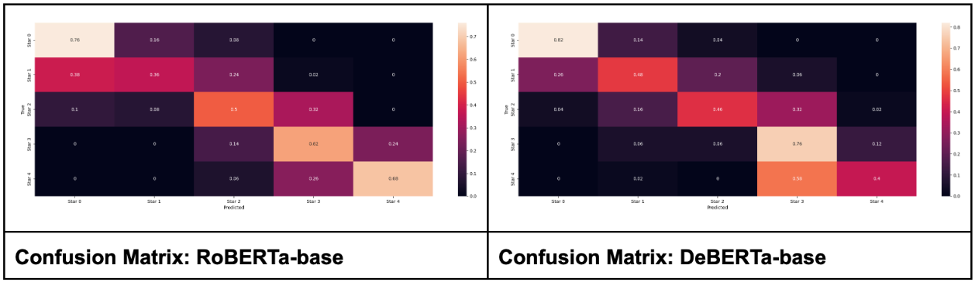
\includegraphics[width=1\textwidth, height=0.2\textheight]{./bert_confusion_matrix.jpg}
  \caption{Confusion matrices for RoBERTa-Base and DeBERTa-base.}
  \label{fig:BERT_confusion}
\end{figure*}

\begin{figure*}[h!]
  \centering
  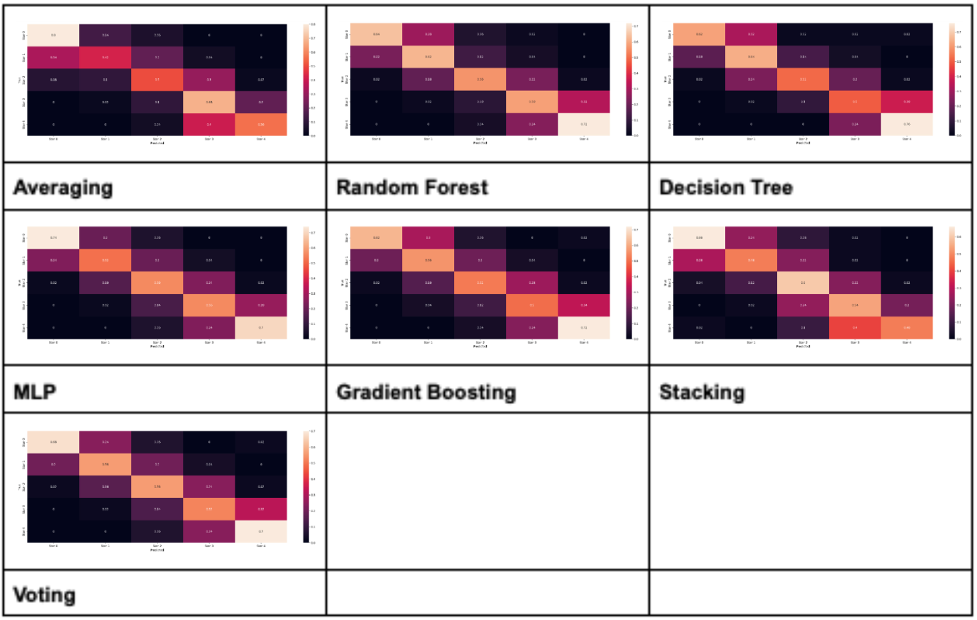
\includegraphics[width=0.8\textwidth, height=0.3\textheight]{./ensemble_confusion_matrix.jpg}
  \caption{Ensemble Confusion Matrices.}
  \label{fig:Ensemble_confusion}
\end{figure*}

\begin{figure*}[h!]
  \centering
  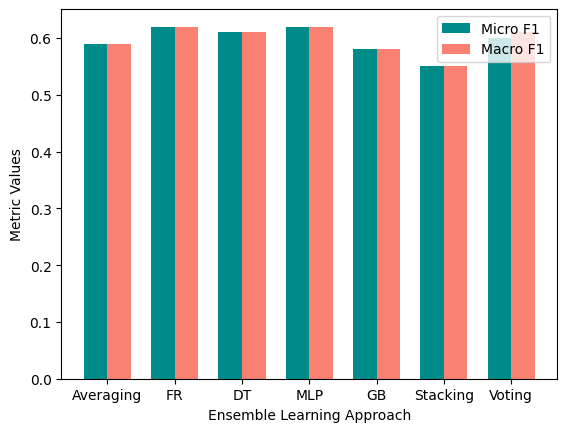
\includegraphics[width=0.8\textwidth, height=0.4\textheight]{./ensemble_chart.jpg}
  \caption{Ensemble Chart Comparison.}
  \label{fig:Ensemble_chart_confusion}
\end{figure*}

\end{document}